%\documentclass[11pt,oneside,a4paper,openright]{report}
%\usepackage[utf8]{inputenc}
%\renewcommand{\contentsname}{Indholdsfortegnelse}
%\usepackage{pdfpages}
%\usepackage{titlesec}
%\titleformat{\chapter}{\normalfont\huge}{\thechapter.}{20pt}{\huge\it}

%%%% Dokumentklassen %%%%

\documentclass[a4paper,11pt,dvipsnames,oneside,openany]{memoir} 	% Openright åbner kapitler på højresider (openany begge)
% fleqn = flush left equation - sikre at alle ligninger tvinges til venstre. I 3. semesterprojektet, skulle ligningerne stå i midten derfor er denne pakke slettet fra dokumentklassen.

\usepackage{subfiles}
\usepackage{nameref}
\usepackage{tabularx}
\usepackage{multirow}
\usepackage[table]{xcolor}


%%%% PACKAGES %%%%

%% Oversættelse og tegnsætning %%
\usepackage[utf8]{inputenc}					% Input-indkodning af tegnsæt (UTF8)
\usepackage[danish]{babel}					% Dokumentets sprog
\usepackage[T1]{fontenc}				    % Output-indkodning af tegnsæt (T1)
\usepackage{ragged2e,anyfontsize}			% Justering af elementer
%\usepackage{fixltx2e}						% Retter forskellige fejl i LaTeX-kernen
\usepackage{titletoc}
\newcommand{\nocontentsline}[3]{}
\newcommand{\tocless}[2]{\bgroup\let\addcontentsline=\nocontentsline#1{#2}\egroup}									% Giver mulighed for at fjerne section nummer i indholdsfortegnelse ved \tocless


\usepackage{lastpage}						% Total antal sider opdateres automatisk ved \pageref{LastPage}
\usepackage{tikz}							% Til at lave flow diagrammer
\usetikzlibrary{calc,trees,positioning,arrows,chains,shapes.geometric,decorations.pathreplacing,decorations.pathmorphing,shapes,matrix,shapes.symbols}				% Til at lave diagrammer
																			
%% Figurer og tabeller (floats) %%
\usepackage{graphicx} 						% Håndtering af eksterne billeder (JPG, PNG, EPS, PDF)
\usepackage{multicol}         	           	% Muliggør output i spalter
\usepackage{rotating}						% Rotation af tekst med \begin{sideways}...\end{sideways}
\usepackage{xcolor}							% Definer farver med \definecolor. Se mere: http://en.wikibooks.org/wiki/LaTeX/Colors
\usepackage{flafter}						% Sørger for at floats ikke optræder i teksten før deres reference
\let\newfloat\relax 						% Justering mellem float-pakken og memoir
\usepackage{float}							% Muliggør eksakt placering af floats, f.eks. \begin{figure}[H]
\usepackage{color, colortbl}				% Tilføjer farve til tabeller

\definecolor{Gray}{gray}{0.9}				% Definerer en farve "yeezy-gray"

%% Matematik mm. %%
\usepackage{amsmath,amssymb,stmaryrd} 		% Avancerede matematik-udvidelser
\usepackage{mathtools}						% Andre matematik- og tegnudvidelser
\usepackage{textcomp}                 		% Symbol-udvidelser (fx promille-tegn med \textperthousand)
\usepackage{rsphrase}						% Kemi-pakke til RS-saetninger, fx \rsphrase{R1}
\usepackage[version=3]{mhchem} 				% Kemi-pakke til flot og let notation af formler, f.eks. \ce{Fe2O3}
\usepackage{siunitx}						% Flot og konsistent præsentation af tal og enheder med \si{enhed} og \SI{tal}{enhed}
\sisetup{output-decimal-marker = {,}}		% Opsætning af \SI (DE for komma som decimalseparator) 

%% Referencer og kilder %%
\usepackage[danish]{varioref}				% Muliggør bl.a. krydshenvisninger med sidetal (\vref)
\usepackage{natbib}							% Udvidelse med naturvidenskabelige citationsmodeller
\usepackage{xr}							    % Referencer til eksternt dokument med \externaldocument{<NAVN>}

%% Misc. %%
\usepackage{listings}						% Placer kildekode i dokumentet med \begin{lstlisting}...\end{lstlisting}
\usepackage{lipsum}							% Dummy text \lipsum[..]
\usepackage[shortlabels]{enumitem}			% Muliggør enkelt konfiguration af lister
\usepackage{pdfpages}						% Gør det muligt at inkludere pdf-dokumenter med kommandoen \includepdf[pages={x-y}]{fil.pdf}	
\pdfoptionpdfminorversion=6					% Muliggør inkludering af pdf-dokumenter, af version 1.6 og højere
\pretolerance=2500 							% Justering af afstand mellem ord (højt tal, mindre orddeling og mere luft mellem ord)


%%%% CUSTOM SETTINGS %%%%

%% Marginer %%
\setlrmarginsandblock{3.0cm}{3.0cm}{*}		% \setlrmarginsandblock{Indbinding}{Kant}{Ratio}
\setulmarginsandblock{3.0cm}{3.0cm}{*}		% \setulmarginsandblock{Top}{Bund}{Ratio}
\checkandfixthelayout 						% Oversætter værdier til brug for andre pakker

%% Afsnitsformatering %%
\setlength{\parindent}{0mm}           		% Størrelse af indryk
\setlength{\parskip}{3mm}          			% Afstand mellem afsnit ved brug af double Enter
\linespread{1,1}							% Linjeafstand

%% Indholdsfortegnelse %%
\setsecnumdepth{subsection}		 			% Dybden af nummererede overskrifter (part/chapter/section/subsection)
\maxsecnumdepth{subsection}					% Dokumentklassens grænse for nummereringsdybde
\settocdepth{subsubsection} 					% Dybden af indholdsfortegnelsen
\setcounter{secnumdepth}{5} 				    % Ekstra subsubsection nummerering
		
%% Opsætning af listings %%
\definecolor{commentGreen}{RGB}{34,139,24}
\definecolor{stringPurple}{RGB}{208,76,239}

\lstset{language=Matlab,				    % Sprog
	basicstyle=\ttfamily\scriptsize,	    % Opsætning af teksten
	keywords={for,if,while,else,elseif,		% Nøgleord at fremhæve
			  end,break,return,case,
			  switch,function},
	keywordstyle=\color{blue},				% Opsætning af nøgleord
	commentstyle=\color{commentGreen},		% Opsætning af kommentarer
	stringstyle=\color{stringPurple},		% Opsætning af strenge
	showstringspaces=false,					% Mellemrum i strenge enten vist eller blanke
	numbers=left, numberstyle=\tiny,		    % Linjenumre
	extendedchars=true, 					    % Tillader specielle karakterer
	columns=flexible,						% Kolonnejustering
	breaklines, breakatwhitespace=true,		% Bryd lange linjer
}

%% Navngivning %%
\addto\captionsdanish{
	\renewcommand\appendixname{Appendiks}
	\renewcommand\contentsname{Indholdsfortegnelse}	
	\renewcommand\appendixpagename{Appendiks}
	\renewcommand\appendixtocname{Appendiks}
	\renewcommand\cftchaptername{\chaptername~}		% Skriver "Kapitel" foran kapitlerne i indholdsfortegnelsen
	\renewcommand\cftappendixname{\appendixname~}	% Skriver "Appendiks" foran appendiks i indholdsfortegnelsen
}

%% Kapiteludssende %%
\definecolor{numbercolor}{gray}{0.7}		            % Definerer en farve til brug til kapiteludseende
\newif\ifchapternonum

\makechapterstyle{jenor}{					        % Definerer kapiteludseende frem til ...
  \renewcommand\beforechapskip{0pt}
  \renewcommand\printchaptername{}
  \renewcommand\printchapternum{}
  \renewcommand\printchapternonum{\chapternonumtrue}
  \renewcommand\chaptitlefont{\fontfamily{pbk}\fontseries{db}\fontshape{n}\fontsize{25}{35}\selectfont\raggedleft}
  \renewcommand\chapnumfont{\fontfamily{pbk}\fontseries{m}\fontshape{n}\fontsize{1in}{0in}\selectfont\color{numbercolor}}
  \renewcommand\printchaptertitle[1]{%
    \noindent
    \ifchapternonum
    \begin{tabularx}{\textwidth}{X}
    {\let\\\newline\chaptitlefont ##1\par} 
    \end{tabularx}
    \par\vskip-2.5mm\hrule
    \else
    \begin{tabularx}{\textwidth}{Xl}
    {\parbox[b]{\linewidth}{\chaptitlefont ##1}} & \raisebox{-15pt}{\chapnumfont \thechapter}
    \end{tabularx}
    \par\vskip2mm\hrule
    \fi
  }
}											        % ... her

\chapterstyle{jenor}						        % Valg af kapiteludseende - Google 'memoir chapter styles' for alternativer

%% Sidehoved %%

\makepagestyle{AAU}							        % Definerer sidehoved og sidefod udseende frem til ...
\makepsmarks{AAU}{%
	\createmark{chapter}{left}{shownumber}{}{. \ }
	\createmark{section}{right}{shownumber}{}{. \ }
	\createplainmark{toc}{both}{\contentsname}
	\createplainmark{lof}{both}{\listfigurename}
	\createplainmark{lot}{both}{\listtablename}
	\createplainmark{bib}{both}{\bibname}
	\createplainmark{index}{both}{\indexname}
	\createplainmark{glossary}{both}{\glossaryname}
}
\nouppercaseheads									% Ingen Caps ønskes

\makeevenhead{AAU}{\small E17BAC-Synk2}{}{\leftmark}	% Definerer lige siders sidehoved (\makeevenhead{Navn}{Venstre}{Center}{Hoejre})
\makeoddhead{AAU}{\rightmark}{}{}		            % Definerer ulige siders sidehoved (\makeoddhead{Navn}{Venstre}{Center}{Højre})
\makeevenfoot{AAU}{\small \thepage \ }{}{ }						% Definerer lige siders sidefod (\makeevenfoot{Navn}{Venstre}{Center}{Højre})
\makeoddfoot{AAU}{}{}{\small \thepage \ }						% Definerer ulige siders sidefod (\makeoddfoot{Navn}{Venstre}{Center}{Højre})

\copypagestyle{AAUchap}{AAU}							% Sidehoved for kapitelsider defineres som standardsider, men med blank sidehoved
\makeoddhead{AAUchap}{}{}{}
\makeevenhead{AAUchap}{}{}{}
\makeheadrule{AAUchap}{\textwidth}{0pt}
\aliaspagestyle{chapter}{AAUchap}					% Den ny style vælges til at gælde for chapters
													% ... her
															
\pagestyle{AAU}										% Valg af sidehoved og sidefod


%%%% CUSTOM COMMANDS %%%%

%% Billede hack %%
\newcommand{\figur}[4]{
		\begin{figure}[H] \centering
			\includegraphics[width=#1\textwidth]{billeder/#2}
			\caption{#3}\label{#4}
		\end{figure} 
}

%% Specielle tegn %%
\newcommand{\decC}{^{\circ}\text{C}}
\newcommand{\dec}{^{\circ}}
\newcommand{\m}{\cdot}


%%%% ORDDELING %%%%

\hyphenation{}


%%%% Tilføjelser af min preample %%%%

% Booktabs:
% The booktabs package is needed for better looking tables. 
\usepackage{booktabs}

% Caption:
% For better looking captions. See caption documentation on how to change the format of the captions.
\usepackage[hang, font={small, it}]{caption}

% Hyperref:
% This package makes all references within your document clickable. By default, these references will become boxed and colored. This is turned back to normal with the \hypersetup command below.
\usepackage{hyperref}
	\hypersetup{colorlinks=false,pdfborder=0 0 0}

% Cleveref:
% This package automatically detects the type of reference (equation, table, etc.) when the \cref{} command is used. It then adds a word in front of the reference, i.e. Fig. in front of a reference to a figure. With the \crefname{}{}{} command, these words may be changed.
\usepackage{cleveref}
	\crefname{equation}{formel}{formler}
	\crefname{figure}{figur}{figurer}	
	\crefname{table}{tabel}{tabeller}

% Mine tilføjelser:
\usepackage{units}                        %% Bruges til at gøre fx 1/2 samlet med: \nicefrac{1}{2}.
\usepackage{tabu, longtable}              %% Bruges til tabeller.
\setlength{\tabulinesep}{1.5ex}           %% Definerer linjeafstand i tabeller.
\usepackage{enumerate}                    %% Bruges til lister.
\usepackage{tabto}                        %% Giver mulighed for TAB med fx \tabto{3em}.
\usepackage[hyphenbreaks]{breakurl}       %% Bruges til websiders url'er.
\renewcommand{\UrlFont}{                  %% Definerer url-font.
\small\ttfamily}                          %
\bibliographystyle{unsrt}                 %% Definere bibliografien. Ses til sidst i dokumentet i kapitlet Litteratur.
\usepackage{amssymb} 
\usepackage{pifont}
%\newcommand{\xmark{\ding{55}}			 % Opretter et unchecked mark

\usepackage[bottom]{footmisc}

\usetikzlibrary{%
    decorations.pathreplacing,%
    decorations.pathmorphing,%
    arrows,
    arrows.meta,
    positioning,
    shapes,
    shadows,
    shapes.geometric
    }
    \usepackage{relsize}

%\definecolor{myblue1}{RGB}{0,157,209}
\definecolor{myblue1}{rgb}{0.12, 0.56, 1.0}
\definecolor{myblue3}{RGB}{216,229,245}
%\definecolor{myblue4}{RGB}{0,149,229}
\definecolor{myblue2}{rgb}{0.19, 0.55, 0.91}
\definecolor{myblue4}{rgb}{0.08, 0.38, 0.74}
\definecolor{myred1}{rgb}{0.82, 0.1, 0.26}
\definecolor{myyellow1}{rgb}{1.0, 0.96, 0.0}
\definecolor{myyellow2}{rgb}{1.0, 0.65, 0.0}


\usepackage{pdflscape}
\usepackage{rotating}

\begin{document}
\begin{titlingpage}
\begin{center}

~ \\[3cm]

%\includegraphics[width=0.6\textwidth]{figurer/ASE}~\\[1cm]

\textsc{\LARGE Bilag 6	}\\[1.5cm]

%\textsc{\Large Sundhedsteknologi}\\
%\textsc{\Large 3. semesterprojekt}\\[0.5cm]

\noindent\makebox[\linewidth]{\rule{\textwidth}{0.4pt}}\\
[0.5cm]{\Huge Implementering \& Test}
\noindent\makebox[\linewidth]{\rule{\textwidth}{0.4pt}}
\end{center}
\vfill
\begin{center}
{\large 19. december 2017}
\end{center}
\end{titlingpage}

\newpage
\tableofcontents*
\newpage

\chapter{Indledning}
I dette bilag beskrives, hvordan de designede hardware og software-komponenter er implementeret og modultestet. På baggrund af disse designede enheder i designfasen foretages der nu implementering og modultest. Til implementering af hardware komponenter er der valgt at opbygge testkredsløbet på et fumlebræt. Hver af disse komponenter skal igennem en modultest for at verificere om de kan bruges til det tiltænkte formål. For softwarens vedkommende dokumenteres, hvordan kodeimplementeringen er foregået, samt resultatet af disse implementeringer. Formålet med modultesten er at forberede produktet til integrationstest.       
\chapter{Implementering}
\section{Hardware}
\subsection{Instrumentationsforstærker 1}
Denne instrumentationsforstærker er tiltænkt til at forstærke et AC signal på 2V til 4V. Til dette formål  er der anvendt instrumentationsforstærkeren INA128 med de begrundelser, som er angivet i designafsnittet. Figur \ref{figScrip} viser INA128 og en eksterne modstand, som bruges til at fastsætte den ønskede forstærkning.  


\begin{figure}[H] 
\centering
{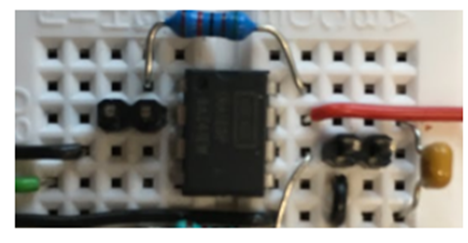
\includegraphics[width=10cm]
{Figure/INA128IM}}
\caption{Figuren viser, hvordan INA128 er implementeret på et fumlebræt  }
\label{figScrip}
\end{figure}



\subsection{Strømgenerator}
Strømgeneratorens funktion er at levere en konstant strøm, som sendes til et måleobjektets væv. Til implementering af denne strømgenerator er der anvendt operationsforstærkeren LM318. Figur \ref{figScrip1}
viser komponenten LM318 med de tilhørende modstande. 
\begin{figure}[H] 
\centering
{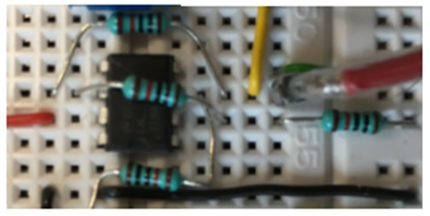
\includegraphics[width=\linewidth]
{Figure/LM318IM}}
\caption{Figuren viser, hvordan LM318 er implementeret på et fumlebræt  }
\label{figScrip1}
\end{figure}


\subsection{Instrumentationsforstærker 2}

Instrumentationsforstærker 2 bliver brugt til at forstærke biosignal fra måleobjektets og undertrykkelse støj . Til implementering af denne Instrumentationsforstærker er der igen brugt INA128. Figur \ref{figINAogSpandeler} B viser komponenten INA128 med dens tilhørende eksterne modstande. Figur \ref{figINAogSpandeler} A viser en spændingsdeler kredsløb, der er benyttet til at teste instrumentationsforstærkeren. Hvorfor der anvendes en spændingsdeler til test af INA128 henvises der til \textit{"bilag 6 - Design"}. 


 

\begin{figure}[H] 
\centering
{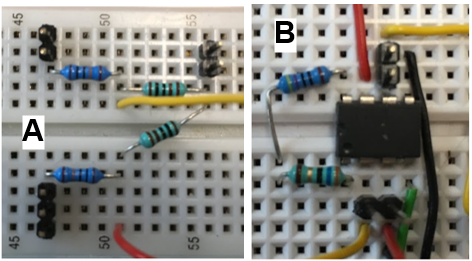
\includegraphics[width=\linewidth]
{Figure/INA128ogSpDelerIM}}
\caption{Figuren viser, hvordan LM318 er implementeret på et fumlebræt  }
\label{figINAogSpandeler}
\end{figure}

\subsection{OP-AMP}

Biosignalet fra måleobjektet forstærkes op i to trin. Det første trin benyttes Instrumentationsforstærker 2 og det andet trin anvendes operationsforstærkeren LM318, som forstærker signalet fra Instrumentationsforstærker 2 yderligere. Figur \ref{opamp} viser implementering af LM318 og de to modstande, som fastsætter, hvor meget forstærkning man kan få ud af operationsforstærkeren. 



\begin{figure}[H] 
\centering
{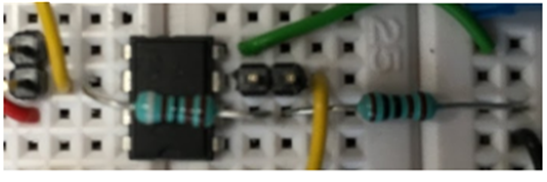
\includegraphics[width=\linewidth]
{Figure/OP-AMPIM}}
\caption{Figuren viser, hvordan LM318 er implementeret på et fumlebræt  }
\label{opamp}
\end{figure}



    
\subsection{Spektrumanalyse}

Der er behov for at foretage en spektrumanalyse, med alle komponenter sat sammen, for at vurdere hvilket krav der skal være til AA filterets dæmpning.  



\begin{figure}[H] 
\centering
{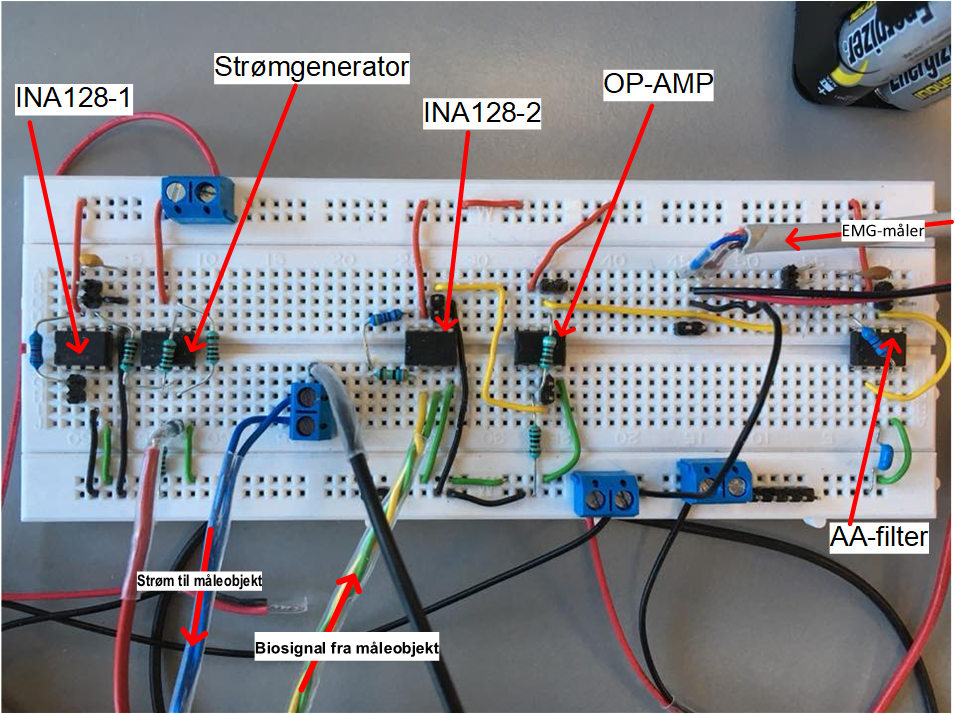
\includegraphics[width=\linewidth]
{Figure/aaspectrumimplementering}}
\caption{Billede over den samlede opstilling med komponenterne: Instrumentationsforstærker 1 \& 2, strømgenerator, OP-AP og monteret elektroder. Disse komponenter repræsentere det samlet frekvensspektrum.}
\label{aaspectrumimplementering}
\end{figure}

\subsection{AA filter}

For at undgå aliasering i det optaget signal implementeres et anti-aliaseringsfilter foran Analog Discovery. AA filteret modtager et forstærketsignal fra OPAMP, filtrere det og sender det videre til Analog Discovery.    

\begin{figure}[H] 
\centering
{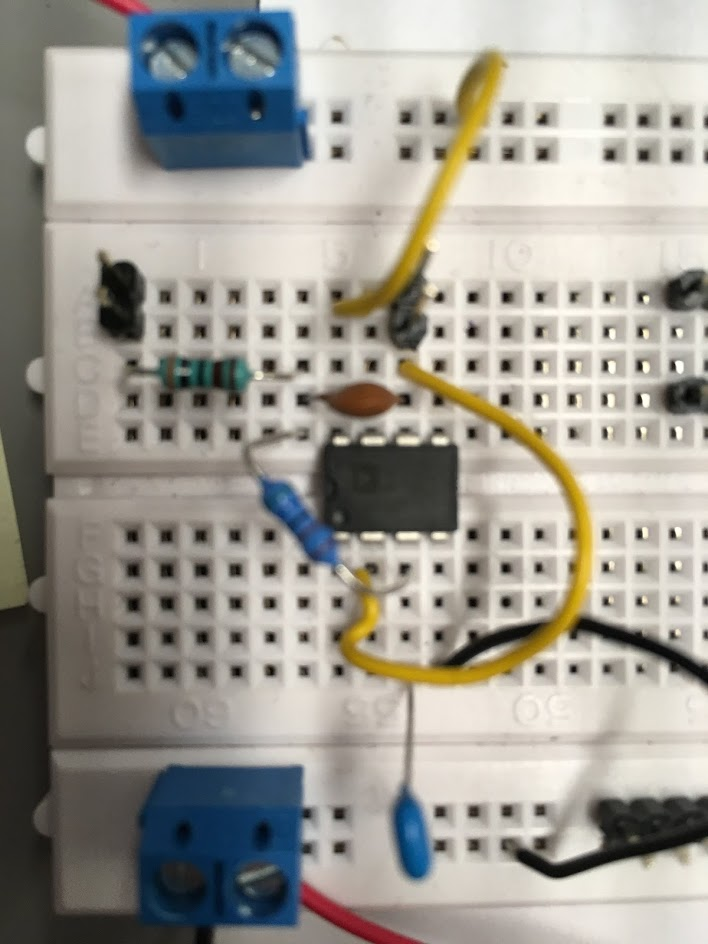
\includegraphics[width=6cm]
{Figure/aafilterimplementering}}
\caption{Implementering af AA filter.}
\label{aafilterimplementering}
\end{figure}





\section{Software}

I dette afsnit beskrives de vigtigste funktioner for systemet software-del. Til implementering af disse funktioner er der brugt udviklingsværktøjet Matlab pga. følgende fordele:

\begin{itemize}
\item  Matlab understøtter styring af Analog Discovery 
\item Matlab forærer databehandlingsfunktioner som ligger klar til anvendelse
\item Matlab er god til at indlæse store mængde data med få kodelinjer
\item I Matlab kan man udvikle en brugergrænseflade nemt og hurtigt 
\item Ved brug af Matlab med Analog Discovery, kan man betjene  funktionsgeneratoren, dataopsamlingsenhed og brugergrænsefladen  fra ét sted   
\end{itemize}  

Alternativet til overnævnte fordele er at man bruger forskellige “single purpose” programmer og enheder, når man skal måle et biomedicinsk signal. \\ \\
I det følgende gennemgås de kritiske funktioner for programmet.

\pagebreak

\subsection{Funktioner}
Funktionernes nærmere beskrivelser henvises der til \textit{"bilag 6 - Design".}

\subsubsection{Synkerefleksmonitor\_OpeningFcn}
\lstinputlisting[frame=single, firstline=48, lastline=50]{matlabkode/Synkerefleksmonitor.m}




\subsubsection{Btn\_Start\_Measurements}
\lstinputlisting[frame=single, firstline=96, lastline=105]{matlabkode/Synkerefleksmonitor.m}


\subsubsection{Btn\_Save\_Measurements}
\lstinputlisting[frame=single, firstline=90, lastline=92]{matlabkode/Synkerefleksmonitor.m}


\subsubsection{Btn\_Load\_Measurements}
\lstinputlisting[frame=single, firstline=154, lastline=164]{matlabkode/Synkerefleksmonitor.m}



\subsubsection{Start\_GUI} 
\lstinputlisting[frame=single]{matlabkode/Start_GUI.m}



\subsubsection{Generate\_SineWave} 

\lstinputlisting[frame=single]{matlabkode/Generate_SineWave.m}



\subsubsection{Read\_Measurements}
\lstinputlisting[frame=single]{matlabkode/Read_Measurements.m}

\subsubsection{Process\_Measurements} 
\lstinputlisting[frame=single]{matlabkode/Process_Measurements.m}




\subsubsection{Show\_Measurements} 
\lstinputlisting[frame=single]{matlabkode/Show_Measurements.m}

\subsubsection{Save\_Measurements} 
\lstinputlisting[frame=single]{matlabkode/Save_Measurements.m}

\subsubsection{Load\_Measurements} 
\lstinputlisting[frame=single]{matlabkode/Load_Measurements.m}

\chapter{Modultest}
Modultest af hardware-delen består af en simuleret test vha. Multisim og en praktisk test. Nogle komponenterne eksister ikke i Multisim og kræver at blive oprettet, men det er valgt at ikke bruge tid på det, da det er tidskrævende. Derfor præsenteres kun praktiske resultater for disse komponenter. I det følgende præsenteres testresultaterne for instrumentationsforstærker 1, 2 , strømgeneratoren, operationsforstærkeren og AA filteret. 

\section{Hardware}

\subsection{Instrumentationsforstærker 1}
Dette modul er testet ved at sende 2V/20kHz fra Analog Discovery (den gule kurve) igennem INA128. Det ses på figur \ref{TestINA} at de 2V bliver forstærket til 4V (turkis kurve) ved udgangen af INA128. Dette resultat stemmer overens med det beregnede resultat i designfasen.    

\begin{figure}[H] 
\centering
{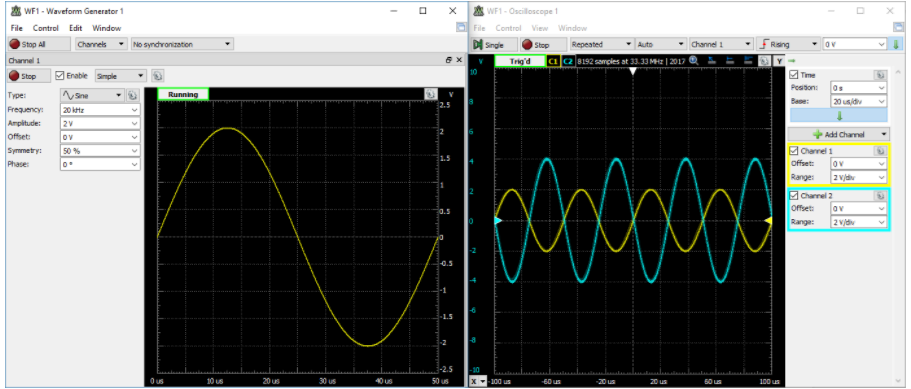
\includegraphics[width=\linewidth]
{Figure/TestINA1281}}
\caption{Figuren viser resultatet af INA128, som forstærker 2V til 4V}
\label{TestINA}
\end{figure}
  \pagebreak
\subsection{Strømgenerator}

Strømgeneratoren er simuleret ved at den får 4V fra en funktionsgenerator. På baggrund af denne spænding genereres der 283uA ud af strømgeneratoren. Bemærk at figur \ref{SimTestStrom} viser strømudgangen ved no-load, hvorimod figur \ref{SimTestStromNoLoad} viser når man belaster strømgeneratoren med $ 10k\Omega$.  

\begin{figure}[H] 
\centering
{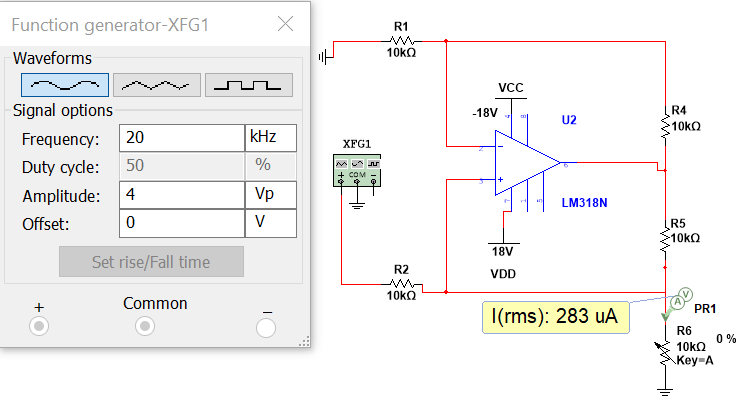
\includegraphics[width=\linewidth]
{Figure/SimuleretStromGenerator}}
\caption{Figuren viser det simuleret resultat for  strømgeneratoren ved no-load}
\label{SimTestStrom}
\end{figure}



\begin{figure}[H] 
\centering
{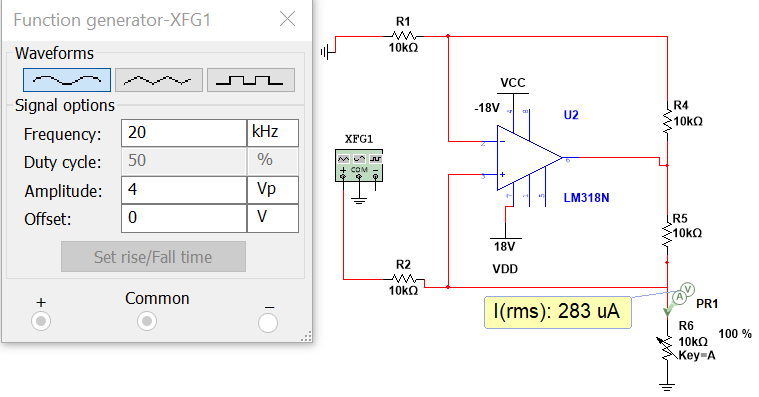
\includegraphics[width=\linewidth]
{Figure/SimuleretStromMedLoad}}
\caption{Figuren viser det simuleret resultat for  strømgeneratoren med load på $10k\Omega$}
\label{SimTestStromNoLoad}
\end{figure}

Det ses på figur \ref{SimTestStromNoLoad} at strømmen ikke ændrer sig, selvom man belaster kredsløbet med $ 10k\Omega	$.   



\pagebreak
Tilsvarende sendes der 4V ind i strømgeneratoren, når der skal foretages den praktiske test på fumlebræt. De 4V genereres fra Analog Discovery. Den producerede strøm måles vha. 
et amperemeter i serie på udgangen af den anvendte operationsforstærker, LM318. Det ses på figur \ref{TestStrGen} at udgangsstrømmen, som genereres af strømgeneratoren er målt til 285uA. Dette resultat afviger lidt fra det beregnede og simulerede resultat. Det vurderes at afvigelsen er så lille at den ingen betydning har for måleobjektets sikkerhed. Figur \ref{fig:Stromgeneratorload} viser strømmens stabilitet fra 1 k$\Omega$ til 10 k$\Omega$, hvilket svarer til området for load impedansen for et biologisk væv \citep{Chester2014}. Derfor er det besluttet at arbejde videre med den målte strøm. 


\begin{figure}[H] 
\centering
{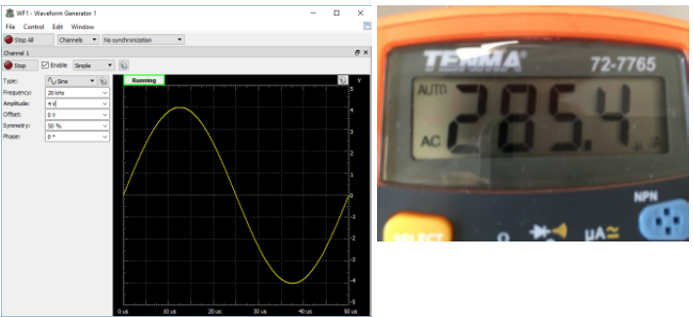
\includegraphics[width=\linewidth]
{Figure/VCCStestParktisk}}
\caption{Figuren viser det praktisk strømresultat som er målt ved udgangen af strømgeneratoren.}
\label{TestStrGen}
\end{figure}

\begin{figure}[H] 
\centering
{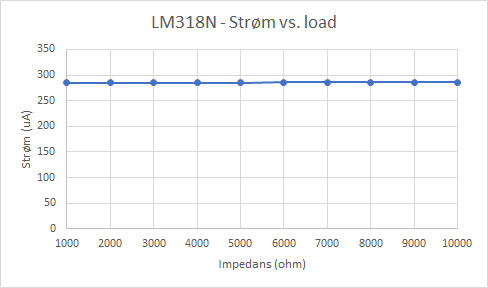
\includegraphics[width=12cm]
{Figure/Stromgeneratorload}}
\caption{}
\label{fig:Stromgeneratorload}
\end{figure}

\subsection{Instrumentationsforstærker 2}

Til test af instrumentationsforstærker 2 er der benyttet en spændingsdeler, som får 1V fra en funktionsgeneratoren, Analog Discovery. Spændingsdelerens funktion er at reducere 1V til 10mV, som efterfølgende forstærkes af instrumentationsforstærker 2 med faktor 100 gange. Som figur \ref{TestAfINA1282} viser, kan man med instrumentationsforstærkeren INA128 opnå en forstærkning på 100. Dette resultat stemmer overens med det teoretiske resultat, som er beregnet i designfasen.  

\begin{figure}[H] 
\centering
{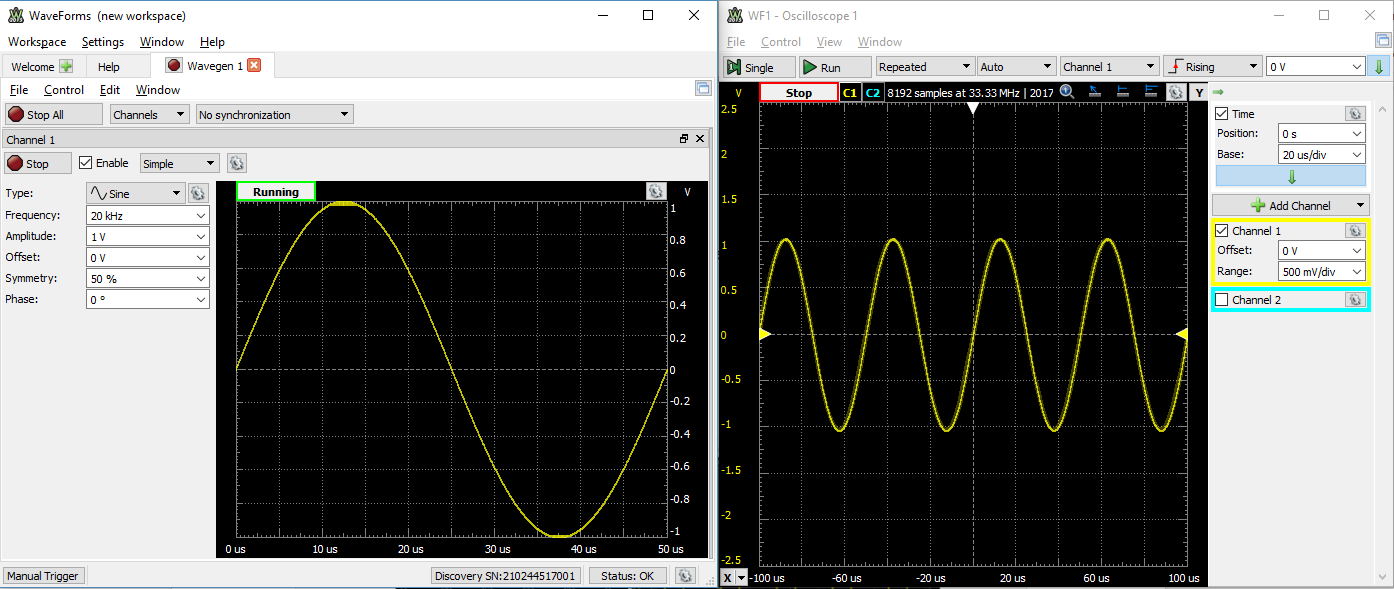
\includegraphics[width=12cm]
{Figure/TestAfINA1282.PNG}}
\caption{Figuren viser det praktiske udgangsspænding for INA128. Denne INA128 yder en forstærkning på 100 gange.}
\label{TestAfINA1282}
\end{figure}






\subsection{OP-AMP}

Denne operationsforstærkers opgave er at forstærke 1 V til 10 V, dvs. en forstærkning ved faktor 10. Der sendes 1V fra funktionsgeneratoren, Analog Discovery, som derefter bliver forstærket til 10 V. Figur \ref{TestAfOpAmp} viser at signalet fra funktionsgeneratoren bliver forstærket 10 gange, dvs. den målte udgangsspænding er på 10V. Hermed stemmer den målte og den teoretiske udgangsspænding af operationsforstærkeren LM318 med hinanden.  

\begin{figure}[H] 
\centering
{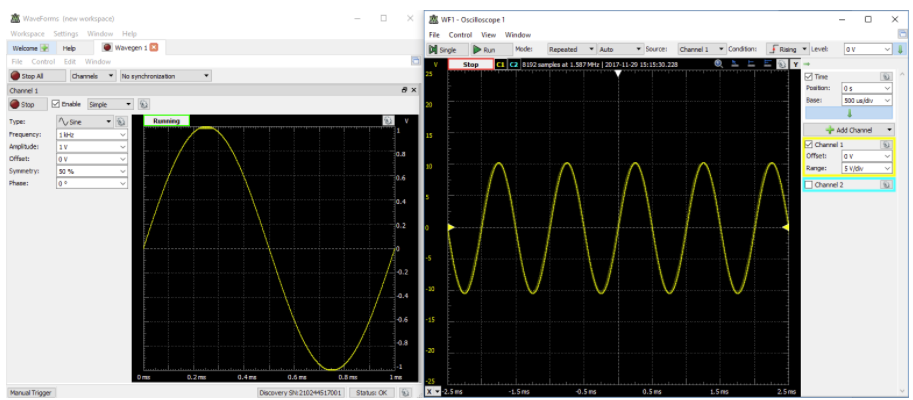
\includegraphics[width=14cm]
{Figure/TestOpamp.PNG}}
\caption{Figuren viser det praktisk udgangsspænding som er målt ved udgangen af operationsforstærkeren.}
\label{TestAfOpAmp}
\end{figure}


\begin{figure}[H] 
\centering
{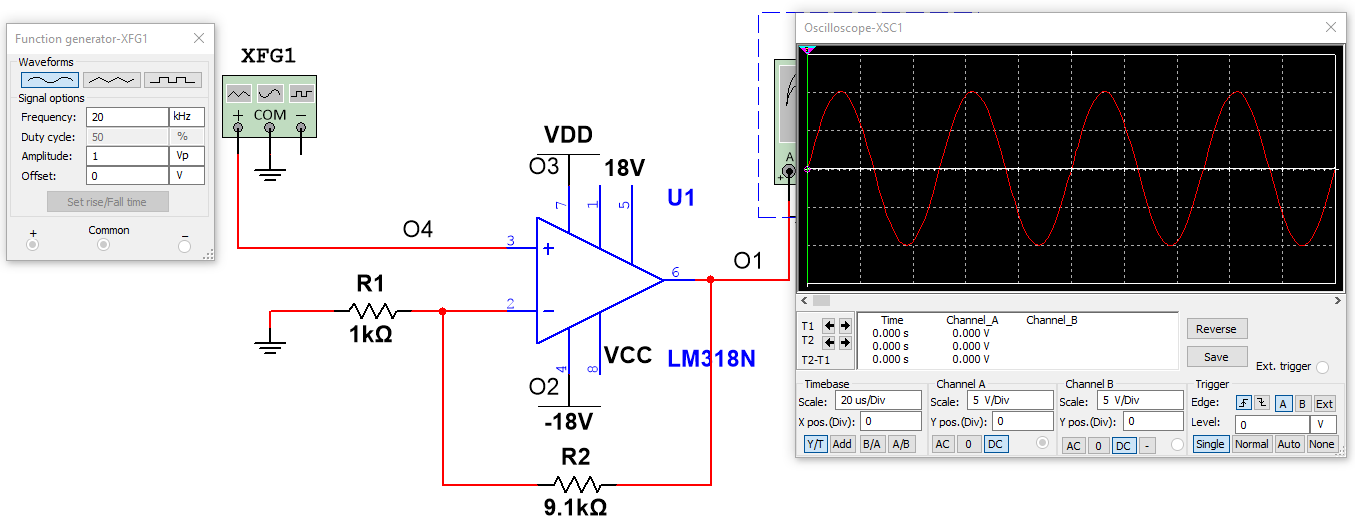
\includegraphics[width=\linewidth]
{Figure/opampmultisim}}
\caption{Figuren viser det simuleret udgangsspænding som er målt ved udgangen af operationsforstærkeren.}
\label{opampmultisim}
\end{figure}


\subsection{Spektrumanalyse}

Ved at sammensætte alle komponenter inkl. elektroder, kan spektrumanalysen blive optaget vha. Analog Discovery. Som det kan aflæses på figur \ref{fig:aaspectrum1}, er der en dæmpning fra det samlet kredsløb på -75 dB. Dette aflæses fra den højeste peak i passbåndet til ca. 250 kHz, som er den halve samplingfrekvens. Da Analog Discovery arbejder med 14bit (skal dæmpe ned til -90 dB) kræver det en yderligere dæmpning på ca. 15 dB. Dette kunne realiseres med et 1. ordens filter, men der vælges at benytte et 2. ordens filter, for at undgå de variationer der måtte være i passbåndet i det målte signal.


\begin{figure}[H] 
\centering
{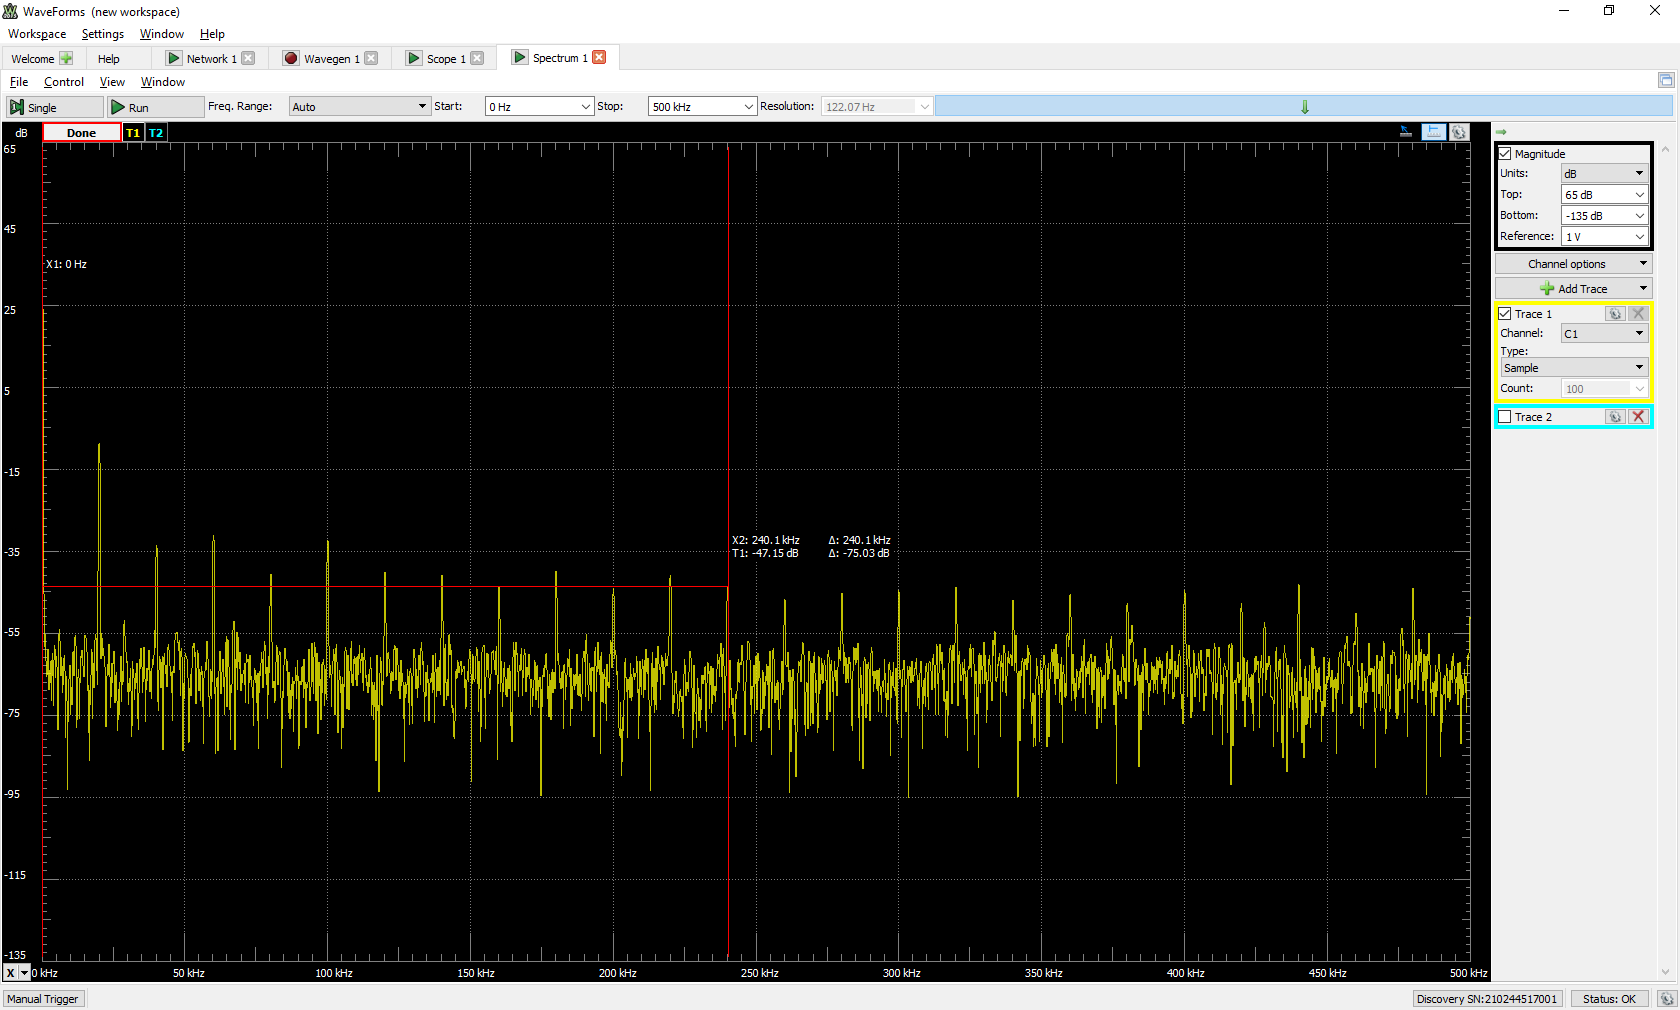
\includegraphics[width=\linewidth]
{Figure/aaspectrum1}}
\caption{Det implementeret frekvensspektrum, som viser at der er en samlet dæmpning på ca. 75dB som skal yderligere dæmpes til 90dB med et 2.ordens lavpasfilter.}
\label{fig:aaspectrum1}
\end{figure}


\subsection{AA filter}

Først er AA filteret simuleret i Multisim. Ved hjælp af Bode Plotter i Multisim, kan det aflæses ved 250 kHz at er en dæmpning på 40 dB.


\begin{figure}[H] 
\centering
{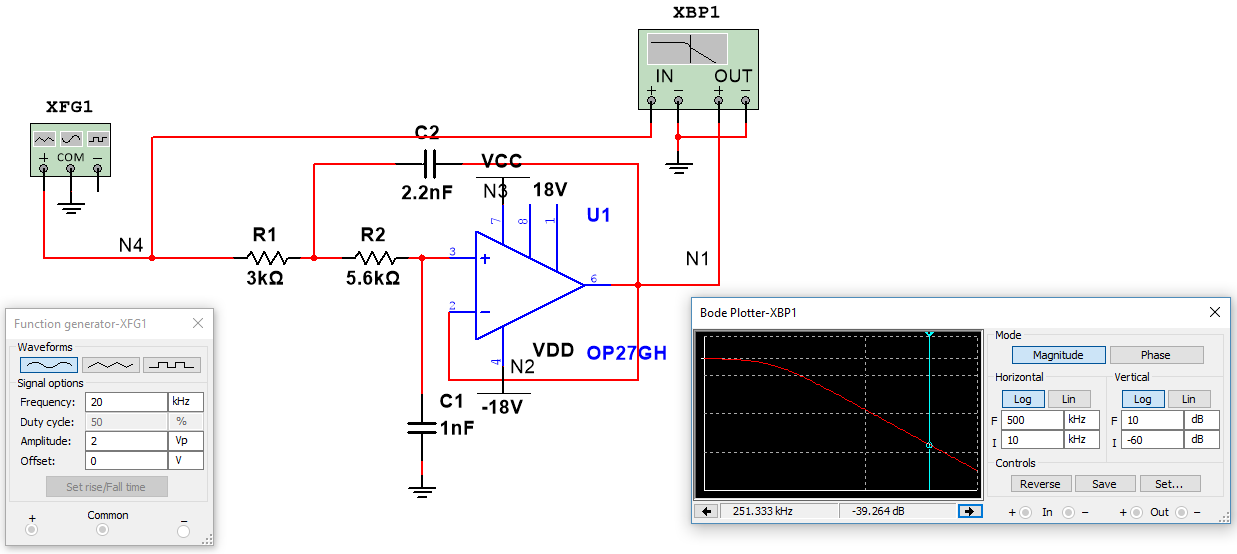
\includegraphics[width=\linewidth]
{Figure/aafilterbodemultisim}}
\caption{Resultat om filterets virkning simuleret i Multisim}
\label{fig:aafilterbodemultisim}
\end{figure}

Der er brugt værktøjet Network Analyzer i programmet Waveforms, for at teste filters virkning, se figur \ref{fig:aafiltermodultest}. Det kan konstateres at ved knækfrekvensen (25 kHz) er faseforskydningen ca. \ang{90}. Efterfølgende kan det aflæses, at ved knækfrekvensen og en dekade frem er der en dæmpning på ca. 35 dB.



\begin{figure}[H] 
\centering
{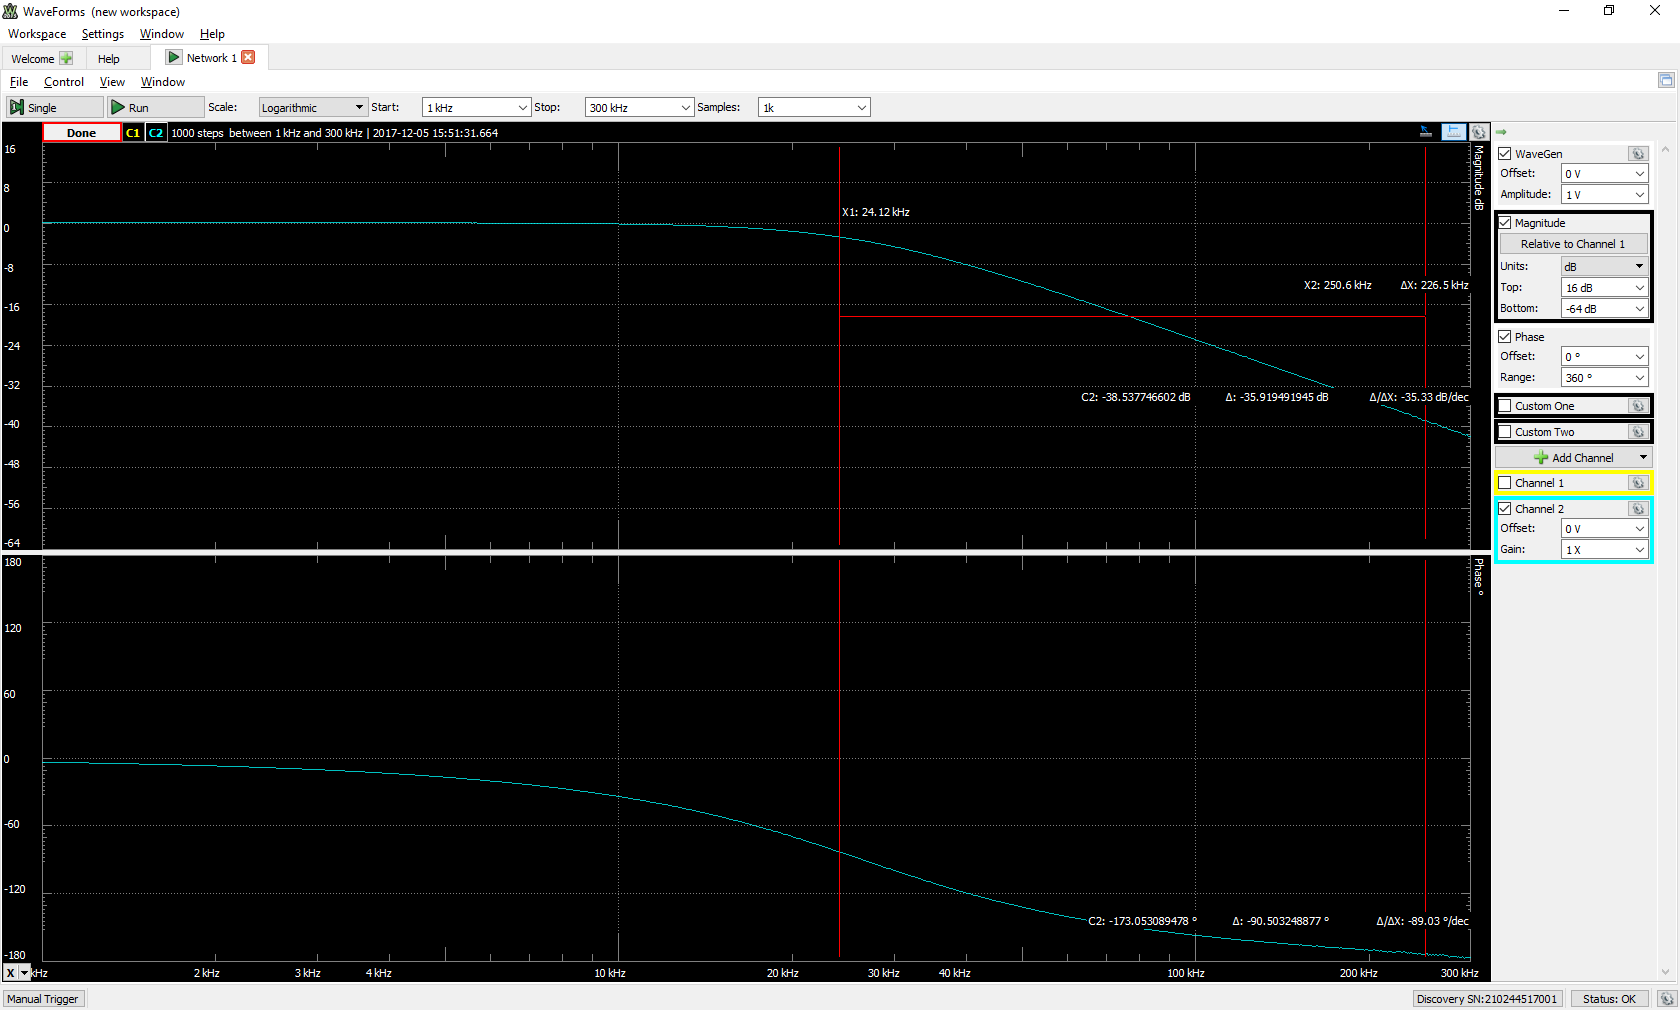
\includegraphics[width=\linewidth]
{Figure/aafiltermodultest}}
\caption{Resultat om filterets virkning fra Network Analyzer i waveforms.}
\label{fig:aafiltermodultest}
\end{figure}





\section{Software}

\subsection{Funktioner}
\subsubsection{Synkerefleksmonitor\_OpeningFcn}








\subsubsection{Btn\_Start\_Measurement}

\begin{figure}[H] 
\centering
{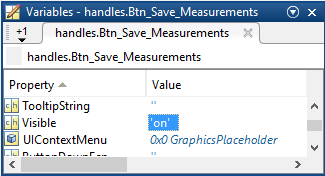
\includegraphics[width=10cm]
{Figure/modultestStart}}
\caption{Oprettelse af dato og tid.}
\label{fig:modultestStart}
\end{figure}


\subsubsection{Btn\_Save\_Measurement}


\subsubsection{Start\_GUI}

Funktionen Start\_GUI køres så snart synkerefleksmonitor.m er startet. Denne funktion har følgende opgaver:
\begin{itemize}
\item Vise dato og tid bliver vist
\item Skjule knappen "Btn\_Save\_Measurement"
\item Vise billede
\end{itemize}

Resultatet af dennes funktions modultest kan ses på figur \ref{fig:modulteststartGUI1}, \ref{fig:modulteststartGUI2} og \ref{fig:modultestGUI}.


\begin{figure}[H] 
\centering
{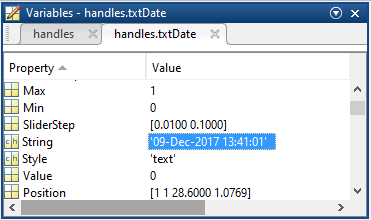
\includegraphics[width=10cm]
{Figure/modulteststartGUI1}}
\caption{Oprettelse af dato og tid.}
\label{fig:modulteststartGUI1}
\end{figure}


\subsubsection{Start\_GUI} 
\begin{figure}[H] 
\centering
{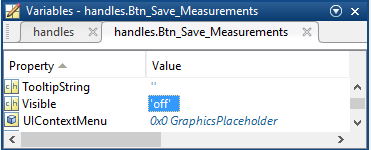
\includegraphics[width=10cm]
{Figure/modulteststartGUI2}}
\caption{Save\_Measurements knappen er gemt fra start.}
\label{fig:modulteststartGUI2}
\end{figure}



\begin{figure}[H] 
\centering
{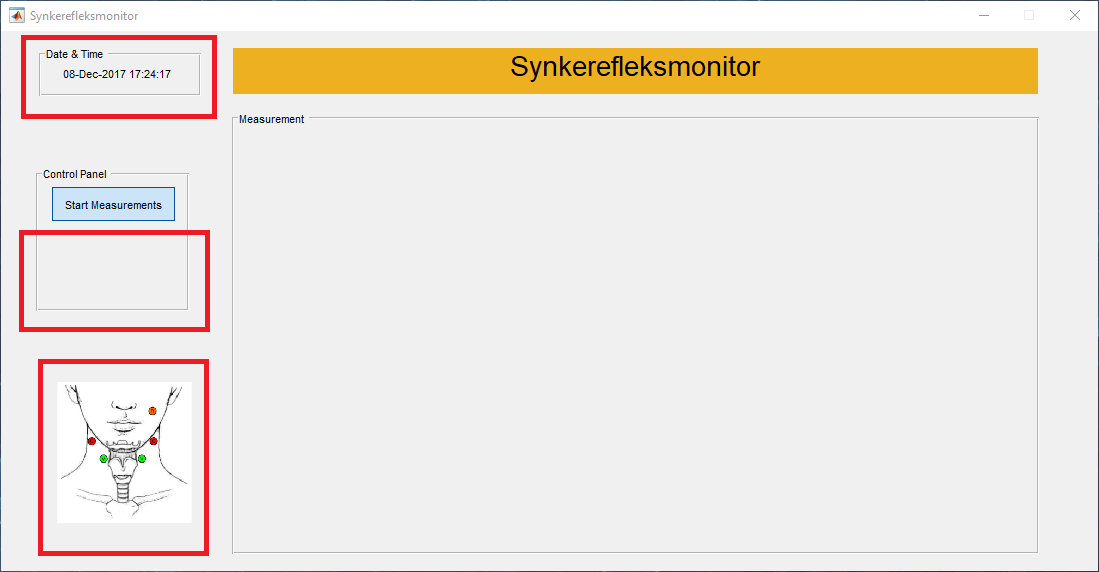
\includegraphics[width=\linewidth]
{Figure/modultestGUI}}
\caption{Resultat fra koden i "Start\_GUI"}
\label{fig:modultestGUI}
\end{figure}


\subsubsection{Generate\_SineWave} 

Funktionen Generate\_SineWave opsætter Analog Discoverys funktionsgenerator. Denne funktion har følgende opgaver:
\begin{itemize}
\item Oprette forbindelse til Analog Discovery
\item Indstille gain til 2 V
\item Indstille frekvensen til 20 kHz
\item Gemme opsætningen i handles.GS
\end{itemize}

Resultatet af dennes funktions modultest kan ses på figur \ref{fig:modultestsinus1}, \ref{fig:modultestsinus3}, \ref{fig:modultestsinus4}, \ref{fig:modultestsinus5} og \ref{fig:modultestsinus}.

\begin{figure}[H] 
\centering
{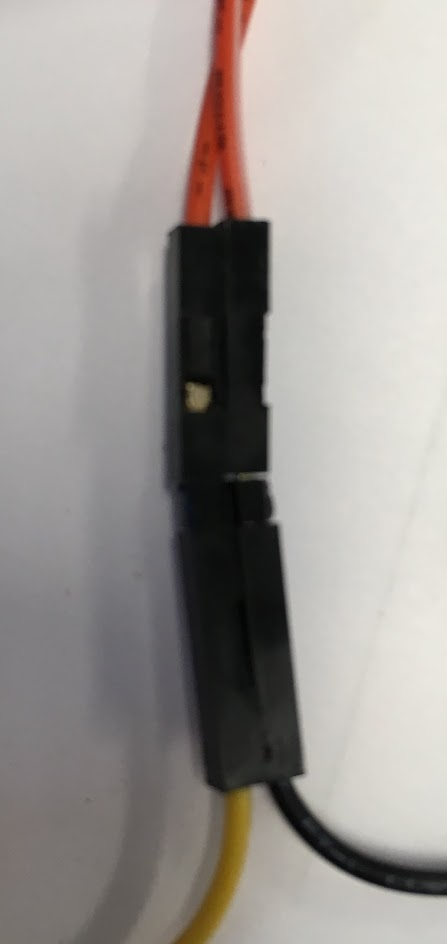
\includegraphics[width=3cm]
{Figure/modultestsinus2}}
\caption{Analog Discoverys funktionsgenerator sættes på Analog Discoverys oscilloskop.}
\label{fig:modultestsinus1}
\end{figure}


\begin{figure}[H] 
\centering
{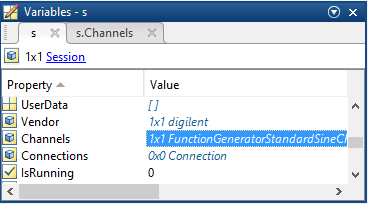
\includegraphics[width=10cm]
{Figure/modultestsinus3}}
\caption{Oprettelsen til Analog Discovery}
\label{fig:modultestsinus3}
\end{figure}



\begin{figure}[H] 
\centering
{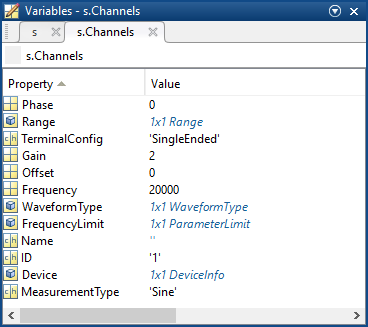
\includegraphics[width=10cm]
{Figure/modultestsinus4}}
\caption{Funktionsgenerator tilføjet.}
\label{fig:modultestsinus4}
\end{figure}

\begin{figure}[H] 
\centering
{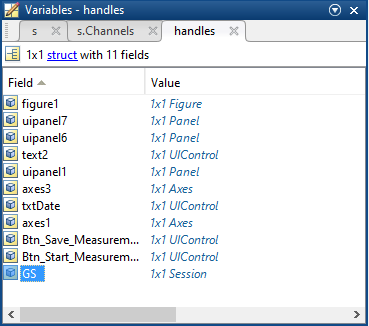
\includegraphics[width=10cm]
{Figure/modultestsinus5}}
\caption{Variablen \textit{"handles.GS"} er oprettet i handles til brug i funktionen \textit{"Read\_Measurements"}.}
\label{fig:modultestsinus5}
\end{figure}



\begin{figure}[H] 
\centering
{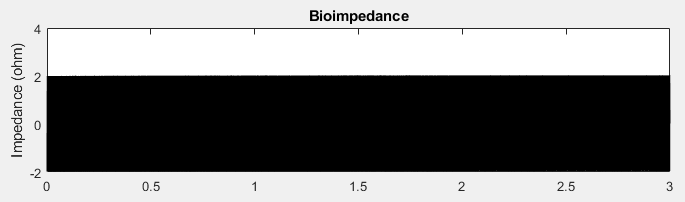
\includegraphics[width=\linewidth]
{Figure/modultestsinus}}
\caption{GUI resultat om koden i "Generate\_SineWave"}
\label{fig:modultestsinus}
\end{figure}







\subsubsection{Read\_Measurements}
Funktionen Read\_Measurements måler BI og EMG signalerne simultant. Denne funktion har følgende opgaver:
\begin{itemize}
\item Indstille tid for måling i sekunder
\item Indstille samplingrate til 500 kHz
\item Oprette to analog input på Analog Discovery
\item Måle BI og EMG simultant
\end{itemize}

Resultatet af dennes funktions modultest kan ses på figur \ref{fig:modultestread3}, \ref{fig:modultestread2}, \ref{fig:modultestread6}, \ref{fig:modultestread7} og \ref{fig:modultestread}.


\begin{figure}[H] 
\centering
{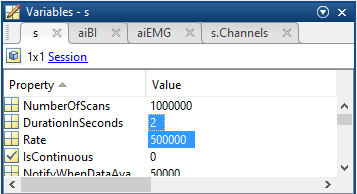
\includegraphics[width=10cm]
{Figure/modultestread3}}
\caption{Indstille sekunder og samplerate.}
\label{fig:modultestread3}
\end{figure}


\begin{figure}[H] 
\centering
{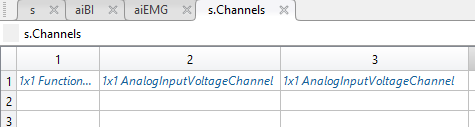
\includegraphics[width=10cm]
{Figure/modultestread2}}
\caption{To analog input oprettet.}
\label{fig:modultestread2}
\end{figure}



\begin{figure}[H] 
\centering
{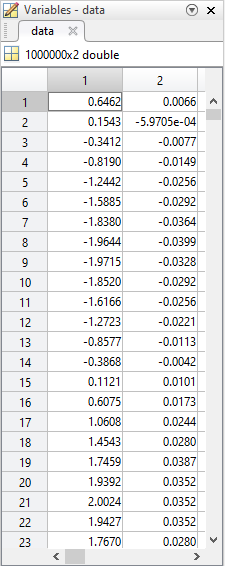
\includegraphics[width=4cm]
{Figure/modultestread6}}
\caption{Målingerne af BI og EMG i tabelform}
\label{fig:modultestread6}
\end{figure}


\begin{figure}[H] 
\centering
{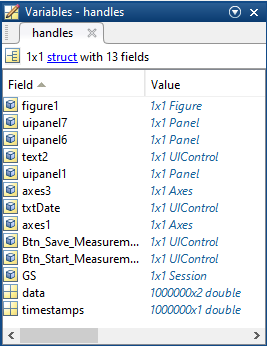
\includegraphics[width=6cm]
{Figure/modultestread7}}
\caption{Målingerne og tiden gemt i handles.}
\label{fig:modultestread7}
\end{figure}



\begin{figure}[H] 
\centering
{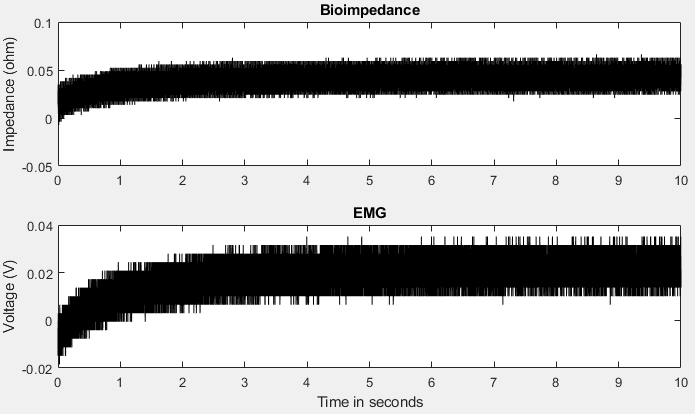
\includegraphics[width=\linewidth]
{Figure/modultestread}}
\caption{Resultat fra koden "Read\_Measurements". To simultane målinger.}
\label{fig:modultestread}
\end{figure}




\subsubsection{Process\_Measurements} 

Funktionen Process\_Measurements behandler BI og EMG målingerne. Denne funktion har følgende opgaver:
\begin{itemize}
\item Dobbelt ensrette BI signal
\item Filtrere BI signal 
\item Oprette to analog input på Analog Discovery
\item Måle BI og EMG simultant
\end{itemize}

Resultatet af dennes funktions modultest kan ses på figur \ref{fig:modultestsinus2}, \ref{fig:modultestprocessSignal}, \ref{fig:modultestprocessEnsrettet}, \ref{fig:modultestprocessFilter} og \ref{fig:modultestprocesshandles}.


\begin{figure}[H] 
\centering
{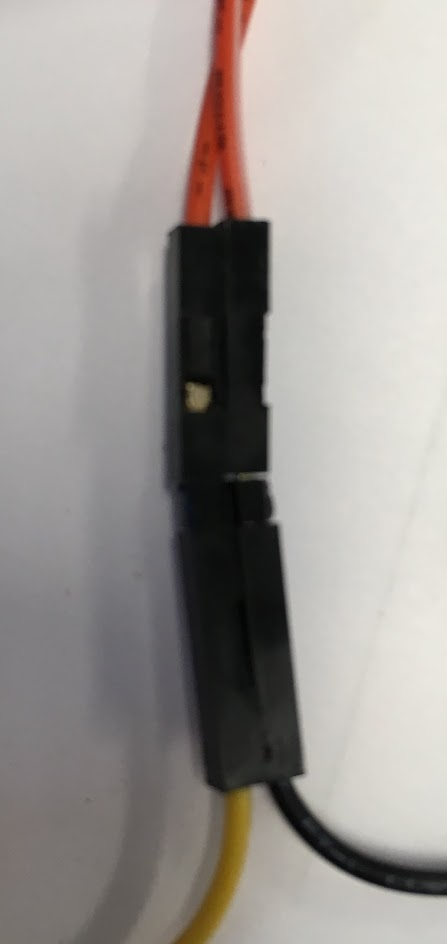
\includegraphics[width=3cm]
{Figure/modultestsinus2}}
\caption{Analog Discoverys funktionsgenerator sættes på Analog Discoverys oscilloskop.}
\label{fig:modultestsinus2}
\end{figure}

\begin{figure}[H] 
\centering
{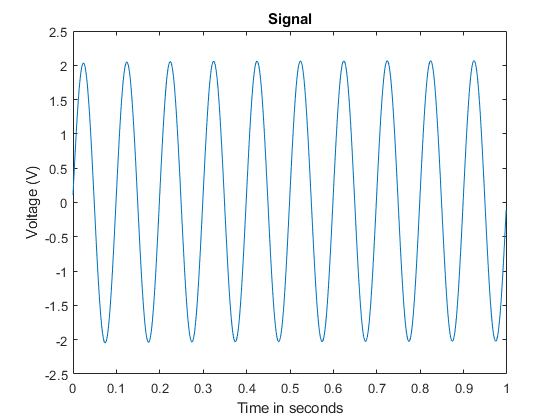
\includegraphics[width=12cm]
{Figure/modultestprocessSignal}}
\caption{Et test BI signal med amplitude på 2 V}
\label{fig:modultestprocessSignal}
\end{figure}

\begin{figure}[H] 
\centering
{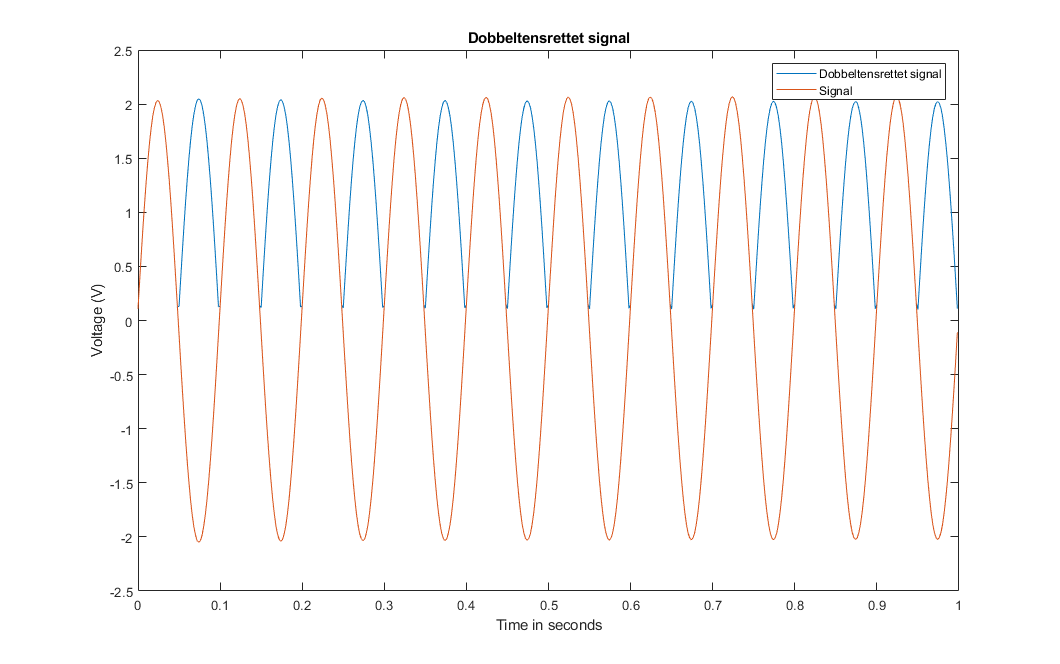
\includegraphics[width=12cm]
{Figure/modultestprocessEnsrettet}}
\caption{BI signalet bliver Dobbelt ensrettet.}
\label{fig:modultestprocessEnsrettet}
\end{figure}


\begin{figure}[H] 
\centering
{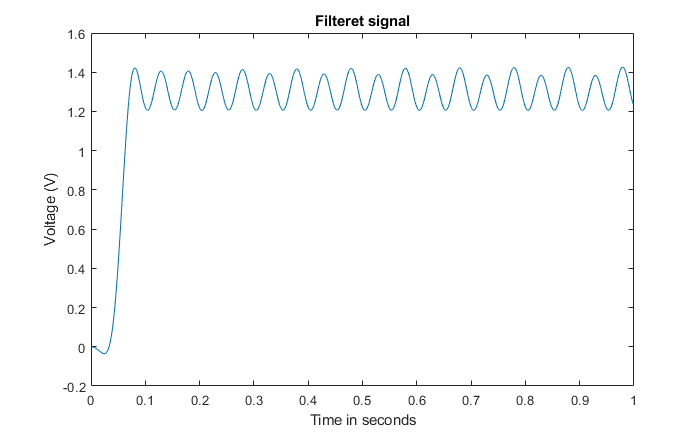
\includegraphics[width=12cm]
{Figure/modultestprocessFilter}}
\caption{BI signalet bliver filteret.}
\label{fig:modultestprocessFilter}
\end{figure}


\begin{figure}[H] 
\centering
{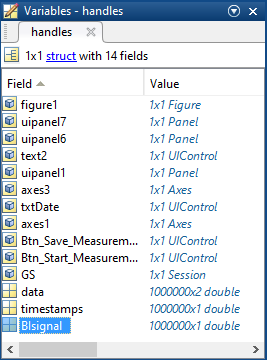
\includegraphics[width=8cm]
{Figure/modultestprocesshandles}}
\caption{Det nye test BI signal gammes i handles.}
\label{fig:modultestprocesshandles}
\end{figure}







\subsubsection{Show\_Measurements} 

Funktionen Show\_Measurements viser de målte BI og EMG signaler simultant. Denne funktion har følgende opgaver:
\begin{itemize}
\item Vise BI og EMG simultant i graf
\end{itemize}

Resultatet af dennes funktions modultest kan ses på figur \ref{fig:modultestshow}.




\begin{figure}[H] 
\centering
{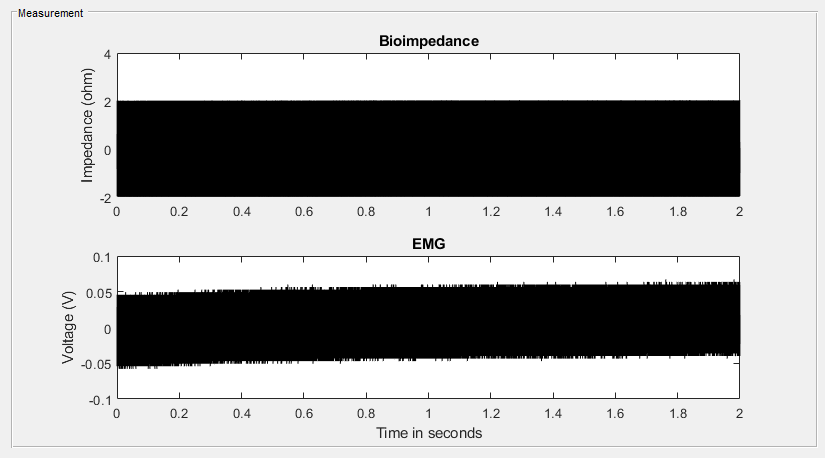
\includegraphics[width=\linewidth]
{Figure/modultestshow}}
\caption{De to simultane test signaler}
\label{fig:modultestshow}
\end{figure}



\subsubsection{Save\_Measurments} 

Funktionen Save\_Measurements gemmer de målte BI og EMG signaler. Denne funktion har følgende opgaver:
\begin{itemize}
\item Gemme BI og EMG signaler i CSV-fil
\end{itemize}

Resultatet af dennes funktions modultest kan ses på figur \ref{fig:modultestsave1} og \ref{fig:modultestsave3}.



\begin{figure}[H] 
\centering
{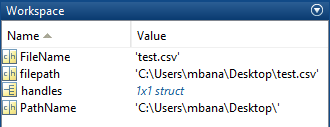
\includegraphics[width=10cm]
{Figure/modultestsave1}}
\caption{Den oprettet sti hvor CSV-filen skal gemmes.}
\label{fig:modultestsave1}
\end{figure}



\begin{figure}[H] 
\centering
{
\includegraphics[width=\linewidth]
{Figure/modultestsave3}}
\caption{Målingen er gemt som test.csv.}
\label{fig:modultestsave3}
\end{figure}


\subsubsection{Load\_Measurments} 

Funktionen Load\_Measurements henter de målte BI og EMG signaler. Denne funktion har følgende opgaver:
\begin{itemize}
\item Hente BI og EMG signaler fra CSV-fil
\end{itemize}

Resultatet af dennes funktions modultest kan ses på figur \ref{fig:modultestLoad1} og \ref{fig:modultestLoad2}.


\begin{figure}[H] 
\centering
{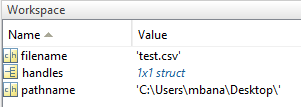
\includegraphics[width=10cm]
{Figure/modultestLoad1}}
\caption{Den oprettet sti hvor CSV-filen skal hentes fra.}
\label{fig:modultestLoad1}
\end{figure}


\begin{figure}[H] 
\centering
{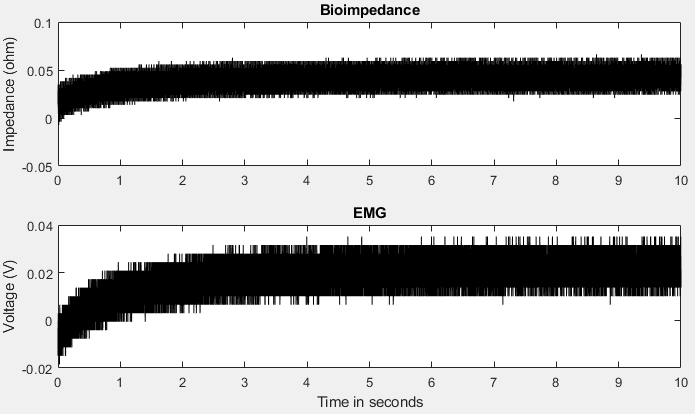
\includegraphics[width=\linewidth]
{Figure/modultestLoad2}}
\caption{De to simultane test signaler er hentet og vises.}
\label{fig:modultestLoad2}
\end{figure}





\chapter{Integrationstest}

\section{Indledning}


Efter modultesten sammensættes de enkelte hardware komponenter gradvist til et færdigt system. I det følgende afsnit dokumenteres ved brug af billeder af opstillingen, multimeter og Analog Discovery. På figur \ref{fig:integrationstestDiagram} er det samlet integreret system inkl. EMG-måler.

\begin{figure}[H] 
\centering
{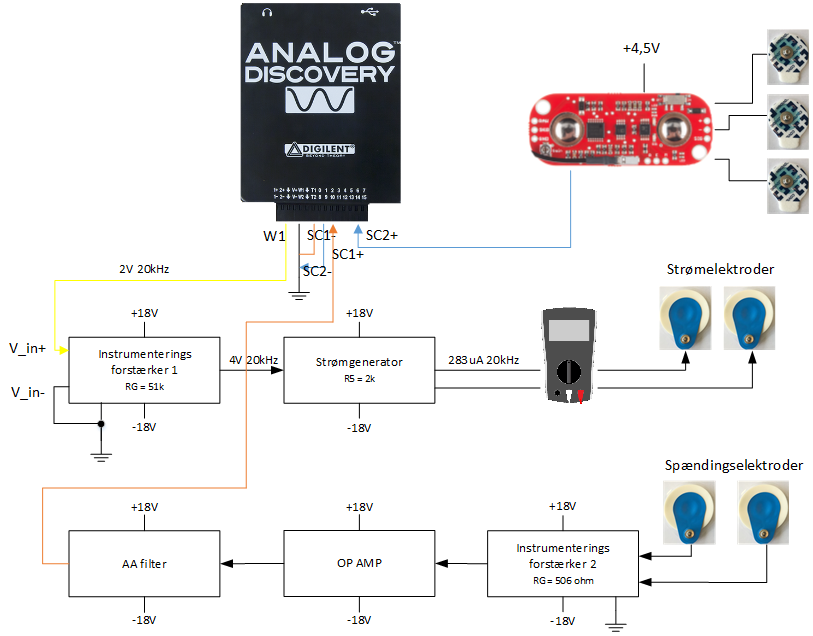
\includegraphics[width=\linewidth]
{Figure/integrationstestDiagram}}
\caption{}
\label{fig:integrationstestDiagram}
\end{figure}


\subsection{Hardware Top-down test}

Ved hjælp af Top-down test styres denne integration af det samlet system som kan ses på figur \ref{fig:integrationstestTopdowntest}. Undervejs er input og output blevet noteret for hver komponent. Forløbet kan ses i tabel \ref{tab:inout}. 

\begin{figure}[H] 
\centering
{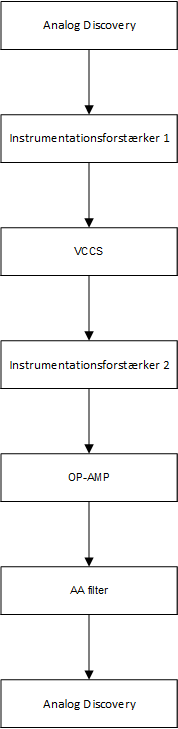
\includegraphics[width=3cm]
{Figure/integrationstestTopdowntest}}
\caption{Top-down test af integrationstesten.}
\label{fig:integrationstestTopdowntest}
\end{figure}

\begin{table}[H]
\center
\begin{tabularx}{\linewidth}{l  X  X X}
     \textbf{Navn}	&	\textbf{Input}		&	\textbf{Output} & \textbf{Kommentar}\\ \midrule
     
     Analog Discovery	&		&	2 V / 20 kHz      & Se figur \ref{fig:integrationstestADud}  \\   \addlinespace[2mm]
     Instrumentationsforstærker 1	&	2 V / 20 kHz	&	4 V / 20 kHz      & Se figur \ref{fig:integrationstestINA1ud}  \\   \addlinespace[2mm]
     VCCS	&	4 V / 20 kHz	&	283 uA / 20 kHz      & Se figur  \ref{fig:integrationstestVCCSud}  \\   \addlinespace[2mm]
     Instrumentationsforstærker 2	&	Biosignal	&	1,67 V      & Se figur  \ref{fig:integrationstestINA2ud}. Strøm faldet til 104 uA, se figur \ref{fig:integrationstestINA2udstrom}  \\   \addlinespace[2mm]
     Op-AMP	&	1,67 V 	&	14,3 V      & Se figur  \ref{fig:integrationstestOPAMPud}  \\   \addlinespace[2mm]	
     AA filter	&	14,3 V 	&	13,4 V      & Se figur  \ref{fig:integrationstestAAud} og for spektrum analyse se figur \ref{fig:integrationstestAAspectrum}.  \\   \addlinespace[2mm]
     \bottomrule                                                                                                                   
    \end{tabularx}
    \caption {Oversigt over input og output for hver komponent, med henvisning enten til figur eller billede.}
    \label{tab:inout}
	
\end{table}


\begin{figure}[H] 
\centering
{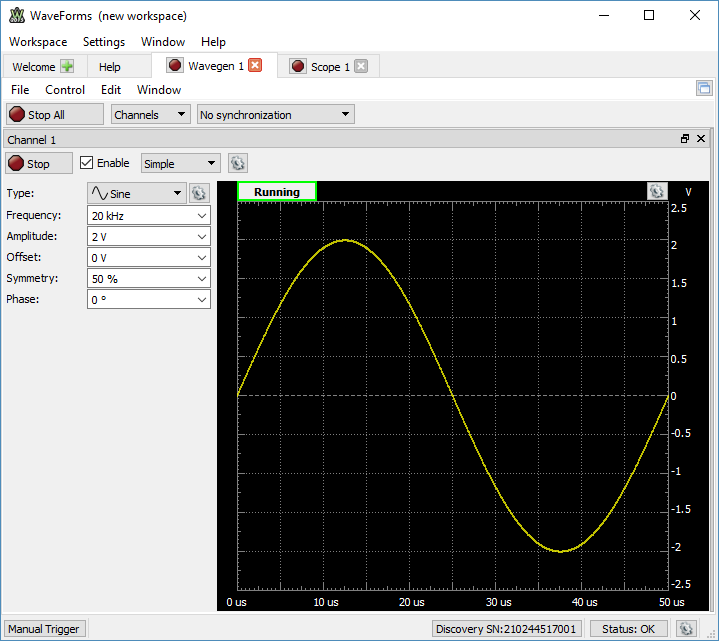
\includegraphics[width=12cm]
{Figure/integrationstestADud}}
\caption{Output på Analog Discovery.}
\label{fig:integrationstestADud}
\end{figure}

\begin{figure}[H] 
\centering
{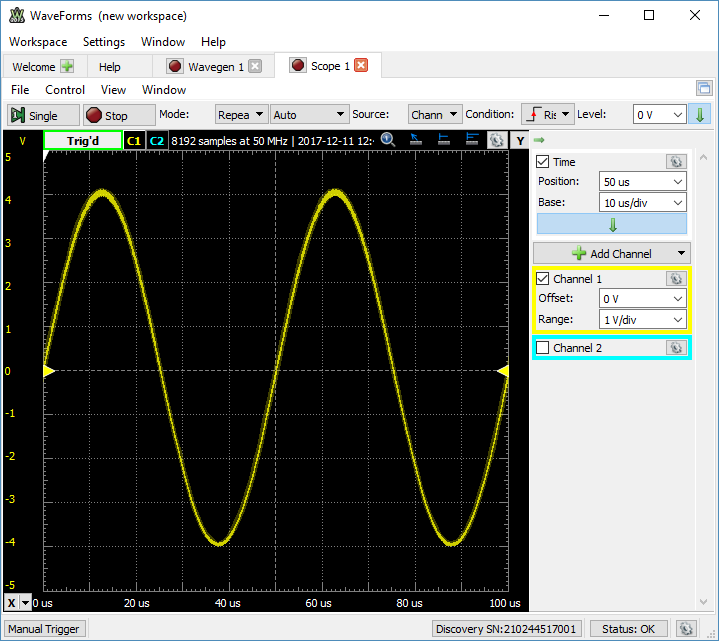
\includegraphics[width=12cm]
{Figure/integrationstestINA1ud}}
\caption{Output på Instrumentationsforstærker 1.}
\label{fig:integrationstestINA1ud}
\end{figure}




\begin{figure}[H] 
\centering
{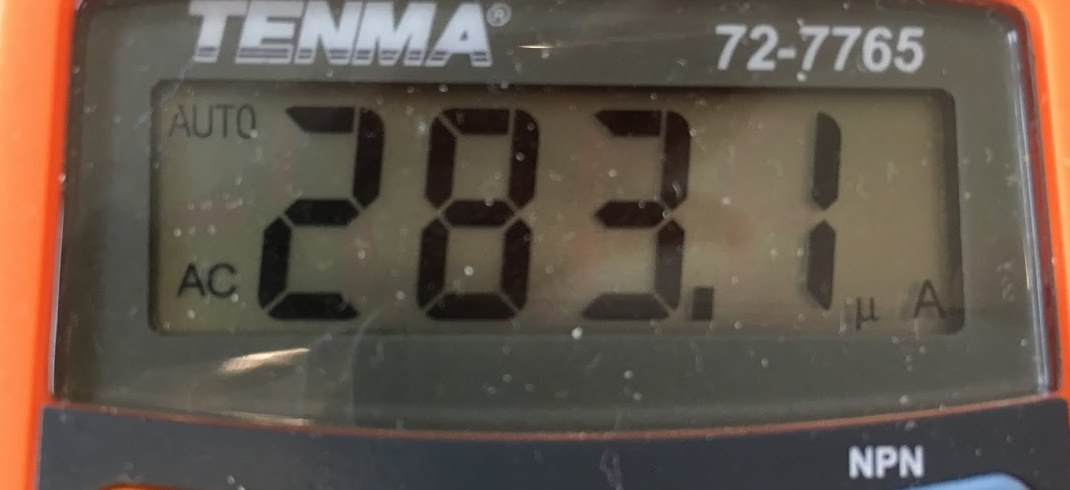
\includegraphics[width=12cm]
{Figure/integrationstestVCCSud}}
\caption{Output på VCCS}
\label{fig:integrationstestVCCSud}
\end{figure}

\begin{figure}[H] 
\centering
{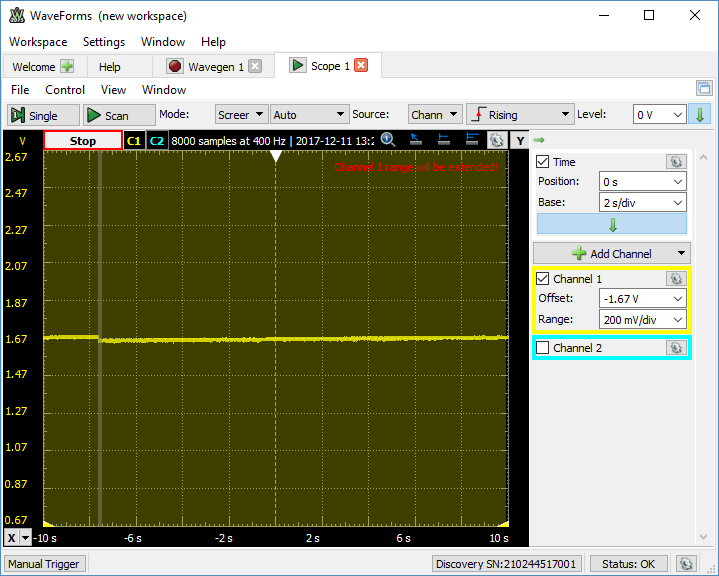
\includegraphics[width=12cm]
{Figure/integrationstestINA2ud}}
\caption{Output på Instrumentationsforstærker 2}
\label{fig:integrationstestINA2ud}
\end{figure}

\begin{figure}[H] 
\centering
{\includegraphics[width=12cm]
{Figure/integrationstestINA2udstrom}}
\caption{Strømmen var faldet til 104 uA fra VCCS, da elektroderne påsættes.}
\label{fig:integrationstestINA2udstrom}
\end{figure}

\begin{figure}[H] 
\centering
{\includegraphics[width=12cm]
{Figure/integrationstestOPAMPud}}
\caption{Output på OP-AMP}
\label{fig:integrationstestOPAMPud}
\end{figure}


\begin{figure}[H] 
\centering
{\includegraphics[width=12cm]
{Figure/integrationstestAAud}}
\caption{Output på AA filter}
\label{fig:integrationstestAAud}
\end{figure}

\begin{figure}[H]
\centering
{\includegraphics[width=\linewidth]
{Figure/integrationstestAAspectrum}}
\caption{Frekvens spektrum af det samlet system. }
\label{fig:integrationstestAAspectrum}
\end{figure} 


\begin{figure}[H]
\centering
{\includegraphics[width=\linewidth]
{Figure/integrationstestBilleder1}}
\caption{Billede af alle komponenter integreret. }
\label{fig:integrationstestBilleder1}
\end{figure} 


\begin{figure}[H]
\centering
{\includegraphics[width=\linewidth]
{Figure/integrationstestBilleder2}}
\caption{Placering af elektroderne uden EMG.}
\label{fig:integrationstestBilleder2}
\end{figure} 


\begin{figure}[H]
\centering
{\includegraphics[width=\linewidth]
{Figure/integrationstestBilleder3}}
\caption{Placering af elektroderne med EMG.}
\label{fig:integrationstestBilleder3}
\end{figure} 

\begin{figure}[H]
\centering
{\includegraphics[width=\linewidth]
{Figure/integrationstestBilleder4}}
\caption{De brugte elektrodeledninger. }
\label{fig:integrationstestBilleder4}
\end{figure} 



Resultatet af integrationstesten, kan også vises i GUI som viser en BI- og EMG-måling simultant på figur \ref{fig:integrationstestSynk1}. 


\begin{figure}[H]
\centering
{\includegraphics[width=\linewidth]
{Figure/integrationstestSynk1}}
\caption{Simultant måling af BI og EMG signal.}
\label{fig:integrationstestSynk1}
\end{figure} 




























\chapter{Accepttest}



\section{Indledning}
Accepttesten skal vise om produktet lever op til de standarder, der er blevet sat op for, at den aktivt kan indgå til klinisk brug. 
Accepttesten er en opfølgning af kravspecifikation, som har til formål at sikre, at alle kravene er overholdt. Der vil blive testet på hovedscenarier. Det er målsætningen, at disse test sikrer produktets kvalitet, idet produktet vil blive afprøvet før det tages i brug. Derfor er det accepttestens ansvarsfunktion, at godkende de opsatte delmål for produktet, hvad angår både funktionelle, samt ikke-funktionelle krav. \\

Når der i feltet Godkendt er et flueben, betyder det at testen er godkendt. Hvis der er et flueben i parenteser, betyder det at den er delvis godkendt. Hvis der er et kryds betyder det, at den ikke er godkendt. 
\section{Accepttest af Usecases}

%Use case 1 acceptest
\subsection{Use Case 1}
Det forventes for Use Case 1, at sundhedspersonalet har fået tilsluttet BI-måleren, EMG-måleren og påsat elektroder på måleobjektet. 

\begin{longtabu} to \linewidth{@{}l r X[j]@{}} %UC1%
	\toprule
	Test af Use Case 1  				&&	Start Measurements\\
	Scenarie 							&&	Hovedscenarie\\
	Prækondition 						&&	Synkerefleksmonitor er monteret korrekt. BI-måleren og EMG-måleren er ledige og operationelle.
Elektroderne påsat måleobjektet og GUI-vinduet er åbent\\ \midrule
\end{longtabu}


\begin{longtabu} to \linewidth{@{} c X[l] X[l] X[j] c@{}}
    ~ &	\textbf{Handling} &    \textbf{Forventet observation/resultat} &		\textbf{Faktisk observation/resultat} &    \textbf{Godkendt}\\[-1ex]
    \midrule
    ~ &\textit{Hovedscenarie} & ~ & ~ &
    \\ \midrule
    1. & Sundhedspersonalet trykker på knappen "Start
Measurements" &   Systemet foretager en måling, hvorefter målingerne vises simultant i graf. &       &	{\Huge \checkmark}	
 \\ \bottomrule
 
\caption{Accepttest af Use Case 1}\\
\label{AT_UC1}
\end{longtabu}

%%%%%%%%%%%%%%%%%%%%%%%%%%%%%%%%%%%%%%%%%%%%%%%%%%%%%%%%%%%%%%%%%%%%%
\subsection{Use Case 2}
\begin{longtabu} to \linewidth{@{}l r X[l]@{}} %UC2%
	\toprule
	Test af Use Case 2  				&&	Save Measurements\\
	Scenarie 							&&	Hovedscenarie\\
	Prækondition 						&&	Use Case 1 er kørt succesfuldt. 
\\ \midrule
\end{longtabu}

\begin{longtabu} to \linewidth{@{} c X[l] X[l] X[j] c@{}}

\setlength{\textfloatsep}{10pt plus 1.0pt minus 2.0pt}
    ~ &	\textbf{Handling} &    \textbf{Forventet observation/resultat} &		\textbf{Faktisk observation/resultat} &    \textbf{Godkendt}\\[-1ex]
    \midrule
    ~ &\textit{Hovedscenarie} & ~ & ~ &
    \\ \midrule
   	1. 	& 	Sundhedspersonalet trykker på knappen "Save
Measurements"	&  Målingerne er gemt i CSV-fil &   &	{\Huge \checkmark}	
    \\
    
 \\ \bottomrule
 
\caption{Accepttest af Use Case 2}\\
\label{AT_UC2}
\end{longtabu}

%%%%%%%%%%%%%%%%%%%%%%%%%%%%%%%%%%%%%%%%%%%%%%%%%%%%%%%%%%%%%%%%%%%%

\subsection{Use Case 3}
\begin{longtabu} to \linewidth{@{}l r X[l]@{}} %UC2%
	\toprule
	Test af Use Case 3  				&&	Load Measurements\\
	Scenarie 							&&	Hovedscenarie\\
	Prækondition 						&&	Use Case 1 og 2 er kørt succesfuldt

\\ \midrule
\end{longtabu}


\begin{longtabu} to \linewidth{@{} c X[l] X[l] X[j] c@{}}
    ~ &	\textbf{Handling} &    \textbf{Forventet observation/resultat} &		\textbf{Faktisk observation/resultat} &    \textbf{Godkendt}\\[-1ex]
    \midrule
    ~ &\textit{Hovedscenarie} & ~ & ~ &
    \\ \midrule
    1. & Sundhedspersonalet trykker på knappen "Load
Measurements " &   Systemet henter målinger og viser i graf  &      & {\Huge \checkmark}

 \\ 
 \bottomrule
 
\caption{Accepttest af Use Case 3}\\
\label{AT_UC3}
\end{longtabu}


\newpage
\section{Accepttest af ikke-funktionelle krav}

\begin{longtabu} to \linewidth{@{} c X[l] X[l] X[j] X[j] c@{}}
	Krav nr. & Krav & Test & Forventet resultat & Resultat & Godkendt
	\\[-1ex] \midrule
	
	1. & Sundheds-personalet skal kunne anvende synkerefleksmonitoren efter 10 minutters instruktion. & Introducér synkerefleksmonitoren & Efter 10 minutter kan Sundhedspersonalet anvende synkerefleksmonitoren & ej testbart & 	\\
2. & Sundheds-personalet skal kunne efter endt introduktion til synkerefleksmonitoren foretage en måling uden stor fejl & Kør Use Case 1 & En måling uden fejl & ej testbart& 	\\ 
3. & Sundheds-personalet skal kunne efter en periode, på 3 måneder væk fra synkerefleksmonitoren, foretage en måling uden fejl & Vent 3 måneder og kør Use Case 1 & En måling uden fejl & ej testbart& 	\\ 
4. & Sundheds-personalet skal kunne aflæse et synk på graferne fra GUI'en på 2 meters afstand. & Sundheds-personalet Sundheds-personalet skal stå to meter væk fra Pc-skærmen & Synket kan ses fra 2 meters afstand& testbart & {\Huge \checkmark}	\\ 

5.& Det skal maksimalt tage 10 minutter(0.17h) at gendanne Synkerefleksmonitor (MTTR - Mean Time To Restore). & Afmontér synkerefleks-monitoren og gendan synkerefleks-monitoren indenfor  10 minutter  & Systemet er funktionelt indenfor 10 minutter & testbart& {\Huge \checkmark}	\\ 
6. & Synkerefleks-monitoren skal have en oppetid uden nedbrud på minimum 1 dag (24 timer)
(MTBF - Mean Time Between Failure)& Tilslut Synkerefleks-monitoren og kør Use case 1,2 og 3 hver time i 24 timer  & Ingen nedbrud efter 1 dag & ej testbart & 	\\ 
7. & Synkerefleks-monitoren skal have en oppetid/køretid på: $Availability = \frac{MTBF}{MTBF+MTTR}\cdot100 = \frac{24}{24+5}\cdot100 = 82,76 \%$& &  & ej testbart & 	\\ 

8. &GUI'ens objekter skal maksimum have en responstid på 30 sekunder & Tryk rundt i GUI og registrer responstid & Responstiden er tilfredsstillende & testbart & {\Huge \checkmark}	\\
9. & Synkerefleks-monitorens hardware skal kunne fungere under temperatur mellem \ang{10}C til \ang{40}C & Synkerefleks-monitorens hardware placeres i \ang{10}C og \ang{40}C  & Synkerefleks-monitoren fungerer& ej testbart & 	\\ 
10. & Sundheds-personalet skal kunne udskifte batterierne til hardwaren inden for 2 minutter &  Sundheds-personalet fjerner batterierne og i sætter nye mens der tages tid & Batterierne er skiftet under 2 minnutter & testbart & {\Huge \checkmark}	\\ 
11. & Sundheds-personalet skal kunne udskifte elektroderne inden for 4 minutter &  Sundheds-personalet fjerner elektroderne og påsætter nye mens der tages tid & Elektroderne er skiftet under 4 minnutter & testbart & {\Huge \checkmark}	\\ 

	\bottomrule
\caption{Accepttest af Ikke-funktionelle krav}
\end{longtabu}







\bibliography{library}
\end{document}
